% Options for packages loaded elsewhere
\PassOptionsToPackage{unicode}{hyperref}
\PassOptionsToPackage{hyphens}{url}
%
\documentclass[
]{book}
\title{Data Science für normale Anwender*innen}
\author{Prof.~Dr.~Nicolas Meseth}
\date{2022-01-12}

\usepackage{amsmath,amssymb}
\usepackage{lmodern}
\usepackage{iftex}
\ifPDFTeX
  \usepackage[T1]{fontenc}
  \usepackage[utf8]{inputenc}
  \usepackage{textcomp} % provide euro and other symbols
\else % if luatex or xetex
  \usepackage{unicode-math}
  \defaultfontfeatures{Scale=MatchLowercase}
  \defaultfontfeatures[\rmfamily]{Ligatures=TeX,Scale=1}
\fi
% Use upquote if available, for straight quotes in verbatim environments
\IfFileExists{upquote.sty}{\usepackage{upquote}}{}
\IfFileExists{microtype.sty}{% use microtype if available
  \usepackage[]{microtype}
  \UseMicrotypeSet[protrusion]{basicmath} % disable protrusion for tt fonts
}{}
\makeatletter
\@ifundefined{KOMAClassName}{% if non-KOMA class
  \IfFileExists{parskip.sty}{%
    \usepackage{parskip}
  }{% else
    \setlength{\parindent}{0pt}
    \setlength{\parskip}{6pt plus 2pt minus 1pt}}
}{% if KOMA class
  \KOMAoptions{parskip=half}}
\makeatother
\usepackage{xcolor}
\IfFileExists{xurl.sty}{\usepackage{xurl}}{} % add URL line breaks if available
\IfFileExists{bookmark.sty}{\usepackage{bookmark}}{\usepackage{hyperref}}
\hypersetup{
  pdftitle={Data Science für normale Anwender*innen},
  pdfauthor={Prof.~Dr.~Nicolas Meseth},
  hidelinks,
  pdfcreator={LaTeX via pandoc}}
\urlstyle{same} % disable monospaced font for URLs
\usepackage{color}
\usepackage{fancyvrb}
\newcommand{\VerbBar}{|}
\newcommand{\VERB}{\Verb[commandchars=\\\{\}]}
\DefineVerbatimEnvironment{Highlighting}{Verbatim}{commandchars=\\\{\}}
% Add ',fontsize=\small' for more characters per line
\usepackage{framed}
\definecolor{shadecolor}{RGB}{248,248,248}
\newenvironment{Shaded}{\begin{snugshade}}{\end{snugshade}}
\newcommand{\AlertTok}[1]{\textcolor[rgb]{0.94,0.16,0.16}{#1}}
\newcommand{\AnnotationTok}[1]{\textcolor[rgb]{0.56,0.35,0.01}{\textbf{\textit{#1}}}}
\newcommand{\AttributeTok}[1]{\textcolor[rgb]{0.77,0.63,0.00}{#1}}
\newcommand{\BaseNTok}[1]{\textcolor[rgb]{0.00,0.00,0.81}{#1}}
\newcommand{\BuiltInTok}[1]{#1}
\newcommand{\CharTok}[1]{\textcolor[rgb]{0.31,0.60,0.02}{#1}}
\newcommand{\CommentTok}[1]{\textcolor[rgb]{0.56,0.35,0.01}{\textit{#1}}}
\newcommand{\CommentVarTok}[1]{\textcolor[rgb]{0.56,0.35,0.01}{\textbf{\textit{#1}}}}
\newcommand{\ConstantTok}[1]{\textcolor[rgb]{0.00,0.00,0.00}{#1}}
\newcommand{\ControlFlowTok}[1]{\textcolor[rgb]{0.13,0.29,0.53}{\textbf{#1}}}
\newcommand{\DataTypeTok}[1]{\textcolor[rgb]{0.13,0.29,0.53}{#1}}
\newcommand{\DecValTok}[1]{\textcolor[rgb]{0.00,0.00,0.81}{#1}}
\newcommand{\DocumentationTok}[1]{\textcolor[rgb]{0.56,0.35,0.01}{\textbf{\textit{#1}}}}
\newcommand{\ErrorTok}[1]{\textcolor[rgb]{0.64,0.00,0.00}{\textbf{#1}}}
\newcommand{\ExtensionTok}[1]{#1}
\newcommand{\FloatTok}[1]{\textcolor[rgb]{0.00,0.00,0.81}{#1}}
\newcommand{\FunctionTok}[1]{\textcolor[rgb]{0.00,0.00,0.00}{#1}}
\newcommand{\ImportTok}[1]{#1}
\newcommand{\InformationTok}[1]{\textcolor[rgb]{0.56,0.35,0.01}{\textbf{\textit{#1}}}}
\newcommand{\KeywordTok}[1]{\textcolor[rgb]{0.13,0.29,0.53}{\textbf{#1}}}
\newcommand{\NormalTok}[1]{#1}
\newcommand{\OperatorTok}[1]{\textcolor[rgb]{0.81,0.36,0.00}{\textbf{#1}}}
\newcommand{\OtherTok}[1]{\textcolor[rgb]{0.56,0.35,0.01}{#1}}
\newcommand{\PreprocessorTok}[1]{\textcolor[rgb]{0.56,0.35,0.01}{\textit{#1}}}
\newcommand{\RegionMarkerTok}[1]{#1}
\newcommand{\SpecialCharTok}[1]{\textcolor[rgb]{0.00,0.00,0.00}{#1}}
\newcommand{\SpecialStringTok}[1]{\textcolor[rgb]{0.31,0.60,0.02}{#1}}
\newcommand{\StringTok}[1]{\textcolor[rgb]{0.31,0.60,0.02}{#1}}
\newcommand{\VariableTok}[1]{\textcolor[rgb]{0.00,0.00,0.00}{#1}}
\newcommand{\VerbatimStringTok}[1]{\textcolor[rgb]{0.31,0.60,0.02}{#1}}
\newcommand{\WarningTok}[1]{\textcolor[rgb]{0.56,0.35,0.01}{\textbf{\textit{#1}}}}
\usepackage{longtable,booktabs,array}
\usepackage{calc} % for calculating minipage widths
% Correct order of tables after \paragraph or \subparagraph
\usepackage{etoolbox}
\makeatletter
\patchcmd\longtable{\par}{\if@noskipsec\mbox{}\fi\par}{}{}
\makeatother
% Allow footnotes in longtable head/foot
\IfFileExists{footnotehyper.sty}{\usepackage{footnotehyper}}{\usepackage{footnote}}
\makesavenoteenv{longtable}
\usepackage{graphicx}
\makeatletter
\def\maxwidth{\ifdim\Gin@nat@width>\linewidth\linewidth\else\Gin@nat@width\fi}
\def\maxheight{\ifdim\Gin@nat@height>\textheight\textheight\else\Gin@nat@height\fi}
\makeatother
% Scale images if necessary, so that they will not overflow the page
% margins by default, and it is still possible to overwrite the defaults
% using explicit options in \includegraphics[width, height, ...]{}
\setkeys{Gin}{width=\maxwidth,height=\maxheight,keepaspectratio}
% Set default figure placement to htbp
\makeatletter
\def\fps@figure{htbp}
\makeatother
\setlength{\emergencystretch}{3em} % prevent overfull lines
\providecommand{\tightlist}{%
  \setlength{\itemsep}{0pt}\setlength{\parskip}{0pt}}
\setcounter{secnumdepth}{5}
\usepackage{booktabs}
\ifLuaTeX
  \usepackage{selnolig}  % disable illegal ligatures
\fi
\usepackage[]{natbib}
\bibliographystyle{plainnat}

\begin{document}
\maketitle

{
\setcounter{tocdepth}{1}
\tableofcontents
}
\hypertarget{uxfcbersicht}{%
\chapter*{Übersicht}\label{uxfcbersicht}}
\addcontentsline{toc}{chapter}{Übersicht}

\hypertarget{zielgruppe}{%
\section*{Zielgruppe}\label{zielgruppe}}
\addcontentsline{toc}{section}{Zielgruppe}

Dieses Buch gibt eine Einführung in wichtige Themen bei der Arbeit mit Daten. Wie der Titel schon ahnen lässt, adressiert dieses Buch \emph{normale} Anwender*innen. Damit meine ich Personen, die in ihrem beruflichen (oder privaten) Alltag von Kenntnissen in der Analyse von Daten (über Excel hinaus) profitieren, diese aber nicht deren Haupttätigkeit ist.

In genau diese Zielgruppe fallen mehr als 95\% der Studierenden, die an der \href{https://hs-osnabrueck.de}{Hochschule Osnabrück} in jedem Semester an meinen Vorlesungen und Seminaren teilnehmen. Sie studieren einen Studiengang aus der Fachrichtung Agrar- oder Lebensmittelwirtschaft und haben in meinen Veranstaltungen die Möglichkeit, zusätzliche Kompetenzen zu digitalen Themen zu entwickeln. Sie arbeiten später aber nicht in IT-Berufen oder als Data Scientist. Sie sind aber dafür gerüstet, mit diesen Abteilungen (IT / Data Scientists) besser zusammenzuarbeiten und viele Dinge können sie auch in Eigenregie umsetzen. Dazu zählen beispielsweise Datenanalysen und -visualisierungen mit R.

\hypertarget{didaktisches-konzept}{%
\section*{Didaktisches Konzept}\label{didaktisches-konzept}}
\addcontentsline{toc}{section}{Didaktisches Konzept}

Das Buch ist in fortlaufend nummerierte Kapitel gegliedert. Man folgt meinem didaktischen Konzept, wenn man diese Reihenfolge einhält. Dieses Konzept beruht darauf, sich zuerst \emph{hands-on} mit einem Thema auseinanderzusetzen, bevor die relevanen theoretischen Hintergründe eingeführt werden. Meiner Erfahrung nach sind theoretische Hintergründe einfacher zu verstehen, wenn das Subjekt der Betrachtung bereits in den Händen war. Der Kontext ist präsent und man weiß bei fachlichen Begriffen sofort die richtige Assoziation herzustellen.

Ein zweiter wichtiger Gedanke beim didaktischen Aufbau des Buches ist die Verwendung von Beispielen aus der Praxis. Dazu zählen insbesodere Datensätze und Fragen an diese Daten. Jedes Kapitel beinhaltet Beispiele und Übungen mit Bezug zu Daten aus der Praxis. Die Anwendungsfälle hinter den Daten reichen von Onlineumfragen aus der Markforschung über Daten aus Laborexperimenten bis hin zu Datensätzen aus sozialen Medien wie Twitter. Alle Datensätze, die in diesem Buch verwendet werden, sind in Kapitel \ref{datensaetze} gelistet.

Nicht immer ist es sinnvoll, ein neues Konzept anhand eines Datensatzes aus der Praxis einzuführen. In diesem Fall greife ich auf synthetische Datensätze zurück, um die Idee oder das Konzept möglichst plastisch darstellen zu können. Die Anwendung des eingeführten Konzepts auf Datensätze aus der Praxis erfolgt dann anschließend. Es sollte in diesem Buch kein Konzept eingeführt werden, das nicht in der Praxis relevant ist.

Das Buch kann selbstverständlich abseits des didaktischen Konzepts verwendet werden. Ich habe beim Verfassen darauf geachtet, das jedes Kapitel in sich geschlossen ist und einzeln gelesen und bearbeitet werden kann. Das gilt auch für die Übungen für die Anwendung mit R.

\hypertarget{part-grundlagen}{%
\part*{Grundlagen}\label{part-grundlagen}}
\addcontentsline{toc}{part}{Grundlagen}

\hypertarget{die-arbeitsumgebung}{%
\chapter{Die Arbeitsumgebung}\label{die-arbeitsumgebung}}

\hypertarget{r-installieren}{%
\section{R installieren}\label{r-installieren}}

R ist eine Open-Source-Software und für alle gängigen Betriebssysteme verfügbar. Ladet euch zunächst die neueste Version von R für euer Betriebssystem herunter und installiert es anschließend:

\begin{itemize}
\tightlist
\item
  \href{https://cran.r-project.org/bin/windows/base/}{R für Windows}
\item
  \href{https://cran.r-project.org/bin/macosx/}{R für macOS}
\item
  \href{https://cran.r-project.org/bin/linux/}{R für Linux}
\end{itemize}

Neben der Sprache und dem Interpreter für R erhaltet ihr mit der Installation auch eine rudimentäre grafische Oberfläche mit dem Namen \emph{RGui} (GUI = Graphical User Interface). Diese besteht aus einer einfachen Konsole, über die ihr R-Befehle eingeben und ausführen könnt.

\begin{figure}
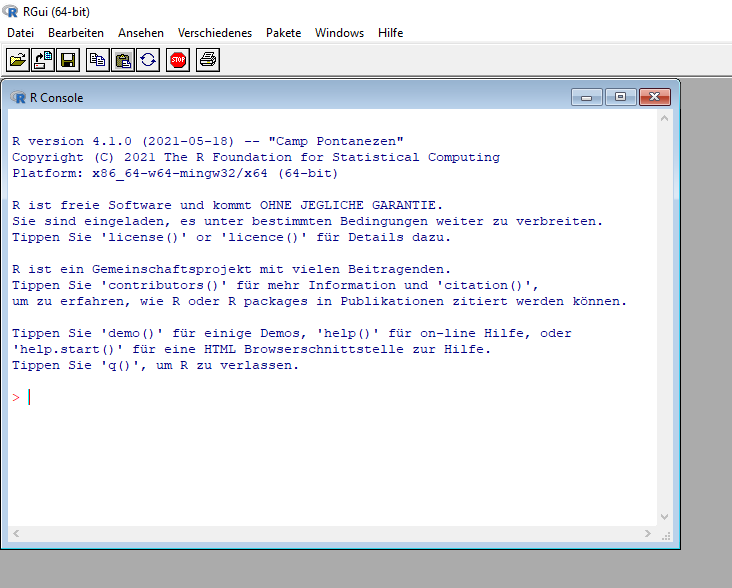
\includegraphics[width=1\linewidth]{fig/screenshot_r_console} \caption{Die RGui bietet einen rudimentären Editor für R-Befehle.}\label{fig:screenshot-r-console}
\end{figure}

Erweiterte Funktionen wie Autovervollständigung beim Schreiben von R-Code, ein integrierter Debugger für die Fehlersuche, eine Echtzeit-Vorschau für R-Markdown und viele andere Features mehr bietet dieses einfache Tool nicht. Deshalb verwenden wir für die Arbeit mit R nicht die RGui, sondern das ebenfalls kostenlos nutzbare \href{https://www.rstudio.com/products/rstudio/}{RStudio}.

\hypertarget{rstudio-installieren}{%
\section{RStudio installieren}\label{rstudio-installieren}}

Das \href{https://www.rstudio.com/}{RStudio} ist das Standardwerkzeug für die Arbeit mit R und bietet dafür viele nützliche Funktionen. Das RStudio ist ein sogenanntes \textbf{Integrated Development Environment (IDE)} für R. Einen schnellen Überblick über die grafische Benutzeroberfläche findet ihr in dem offiziellen \href{https://raw.githubusercontent.com/rstudio/cheatsheets/main/rstudio-ide.pdf}{RStudio Cheatsheet}.

Klickt auf den Link unten und wählt RStudio für euer Betriebssystem aus. Installiert RStudio und öffnet es:

\begin{itemize}
\tightlist
\item
  \href{https://www.rstudio.com/products/rstudio/download/\#download}{RStudio herunterladen}
\end{itemize}

Nach dem Öffnen seht ihr die Oberfläche des RStudio, die wie auf dem Screenshot unten aussieht:

\begin{figure}
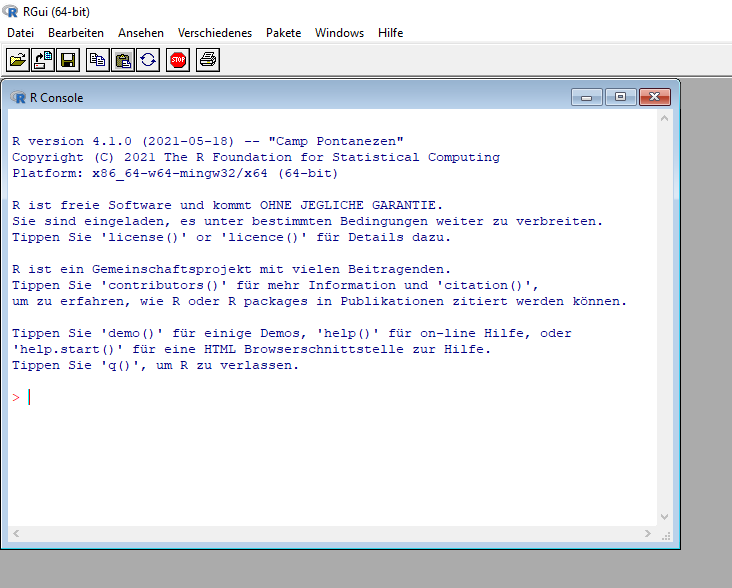
\includegraphics[width=1\linewidth]{fig/screenshot_r_console} \caption{Das RStudio ist in vier Bereiche eingeteilt.}\label{fig:screenshot-rstudio}
\end{figure}

\hypertarget{uxfcberblick-uxfcber-rstudio}{%
\section{Überblick über RStudio}\label{uxfcberblick-uxfcber-rstudio}}

Das Werkzeug besteht in der Standardansicht aus vier Bereichen (s. Screenshot oben):

\hypertarget{der-skripteditor}{%
\subsection{Der Skripteditor}\label{der-skripteditor}}

Der wichtigste Bereich ist der Skripteditor. Hier schreiben wir unseren R-Code und speichern ihn in Dateien auf unserem Computer. Dabei unterstützt uns RStudio mit vielen nützlichen Funktionen.

Wir können in RStudio unterschiedliche Arten von Dateien verwenden, um unsere Skripte zu speichern. Die einfachste Art sind sogenannte R-Skripte mit der Dateiendung \texttt{.R}. Wenn wir nicht nur R-Code, sondern auch Visualisierungen und formatierten Text in einem Dokument verwenden wollen, bietet sich die Verwendung eines R-Notebooks an. Ein R-Notebook endet auf \texttt{.Rmd} und wir können neben R-Code auch Markdown verwenden.

\hypertarget{informationen-zur-aktuellen-r-umgebung}{%
\subsection{Informationen zur aktuellen R-Umgebung}\label{informationen-zur-aktuellen-r-umgebung}}

R erstellt für die Ausführung von Skripten eine sogenannte Session. In einer Session werden alle Objekte, wie die momentan verwendeten Daten, eigene Variablen oder Funktionen, im Arbeitsspeicher des lokalen Rechners gespeichert. In dem zweiten Fenster können im Tab \emph{Environment} alle Objekte, die es in der aktuellen Session gibt, in der Übersicht und im Detail betrachtet werden. Der \emph{History} Tab enthält eine Liste aller ausgeführten Befehle in der aktuellen Session. Daneben gibt es noch den \emph{Connections} Tab für die Verbindung zu unterschiedlichen Datenquellen, wie Datenbanken oder Webservices, sowie den \emph{Tutorial} Tab, in dem direkt in RStudio unterschiedliche Anleitungen angezeigt werden können.

\{\% hint style=``info'' \%\}
Für die Anzeige von Tutorials direkt in RStudio muss das Paket \texttt{learnr} installiert werden. Ihr müsst der Installation einmalig zustimmen und das Paket installieren.
\{\% endhint \%\}

\hypertarget{konsole-und-terminal}{%
\subsection{Konsole und Terminal}\label{konsole-und-terminal}}

Die Konsole ermöglicht, R-Befehle einzugeben und mit der Taste Enter auszuführen. Die Konsole in RStudio ist fast identisch zu der RGui. Für das schnelle Ausprobieren von Befehlen kann die Konsole nützlich sein. Für die strukturierte Arbeit mit den Daten sollten wir aber den Skripteditor verwenden, weil wir dort unsere Arbeit speichern und mit Kommentaren versehen können.

\hypertarget{dateien-vorschau-und-plots}{%
\subsection{Dateien, Vorschau und Plots}\label{dateien-vorschau-und-plots}}

In diesem Bereich werden Vorschauen unterschiedlicher Artefakte angezeigt. Dazu gehören gerenderte R-Notebooks, Markdown, aber auch Visualisierungen. In diesem Bereich gibt es auch einen rudimentären Datei-Explorer, um Dateien wie Skripte oder Datendateien zu finden und von dort zu öffnen.

\hypertarget{strukturierte-daten-tabellen}{%
\chapter{Strukturierte Daten (Tabellen)}\label{strukturierte-daten-tabellen}}

Nachdem die Arbeitsumgebung eingerichtet ist können wir mit den ersten Schritten in R beginnen. Wir steigen direkt ein und lernen, wie wir mit Daten in R arbeiten.

\hypertarget{der-dataframe}{%
\section{Der Dataframe}\label{der-dataframe}}

In R gibt es verschiedene Strukturen für die Speicherung von Daten. Darunter sind beispielsweise Vektoren, Listen oder Matritzen. Um tabellarische Daten abzubilden, die in Spalten und Zeilen organisiert sind, verwenden wir in R den sogenannten \textbf{Dataframe}.

\hypertarget{tibbles}{%
\section{Tibbles}\label{tibbles}}

Wenn man so will ist der Tibble eine Weiterentwicklung des klassischen Dataframe in R. Tibbles werden im Tidyverse standardmäßig verwendet und mit dem Paket \texttt{tibble} eingeführt.

\hypertarget{daten-aus-dem-csv-format-laden}{%
\chapter{Daten aus dem CSV-Format laden}\label{daten-aus-dem-csv-format-laden}}

\hypertarget{das-csv-format}{%
\section{Das CSV-Format}\label{das-csv-format}}

In den meisten Fällen erzeugen wir einen Dataframe oder Tibble, indem wir einen Datensatz aus einer Datenquelle laden. Häufig ist die Quelle eine einfache Texdatei, in der Daten zeilenweise gespeichert sind und jede Zeile aus mehreren Werten besteht, die durch ein Trennzeichen voneinander getrennt sind. Wenn die Werte mit einem Komma voneinander getrennt sind, nennt man das Forat auch \textbf{CSV}. CSV steht für \textbf{Comma Separated Values}, was auf Deutsch so viel wie \emph{Durch Kommata getrennte Werte} bedeutet.

\hypertarget{einen-datensatz-erkunden}{%
\chapter{Einen Datensatz erkunden}\label{einen-datensatz-erkunden}}

\hypertarget{alle-daten-anzeigen}{%
\section{Alle Daten anzeigen}\label{alle-daten-anzeigen}}

Oft ist es hilfreich, einen schnellen Blick in einen Datensatz zu werfen, um beispielsweise die Werte einer Spalte zu überprüfen. Dafür können wir in RStudio die Funktion \texttt{view()} verwenden. Der Funktion übergeben wir ein Tibble und es öffnet sich daraufhin ein neuer Tab im Skripteditor, der die Daten als Tabelle anzeigt.

\begin{Shaded}
\begin{Highlighting}[]
\FunctionTok{view}\NormalTok{(food\_production)}
\end{Highlighting}
\end{Shaded}

\hypertarget{datensaetze}{%
\chapter{Datensätze}\label{datensaetze}}

\begin{longtable}[]{@{}
  >{\raggedright\arraybackslash}p{(\columnwidth - 4\tabcolsep) * \real{0.51}}
  >{\raggedright\arraybackslash}p{(\columnwidth - 4\tabcolsep) * \real{0.33}}
  >{\raggedright\arraybackslash}p{(\columnwidth - 4\tabcolsep) * \real{0.16}}@{}}
\caption{Datensätze in diesem Buch}\tabularnewline
\toprule
\endhead
\textbf{Name} & \textbf{Download-Link} & \textbf{Kategorie} \\
Online-Umfrage zum Kaufverhalten von Orangenlimonade & \href{datasets/limonade.csv}{Download} & Marktforschung \\
Tweets ausgewählter deutscher Politiker:innen & Download & Soziale Medien \\
& & \\
\bottomrule
\end{longtable}

  \bibliography{book.bib,packages.bib}

\end{document}
